\documentclass[english]{article}
\usepackage{packages}
\usepackage{algpseudocode}
\addbibresource{bibfile.bib}
\usepackage{times}
\linenumbers 

\begin{document}
   \author*[1]{JOSE ARMANDO SON ROJAS}
  \runningauthor{AUTHOR 1}
%  \affil[1]{AFFILIATION 1}
  \title{Visualizaciòn Cientifica}
  \subtitle{Algoritmo de Relevo en Ciclismo}
  \abstract{Se va implementar un algoritmo de relevo en Ciclismo segùn los conceptos vistos en clases, teniendo en cuenta Taxonomia, Interacciones, Vectores de Algoritmos, entre otros temas}

\maketitle  

\section{Conceptos Bàsicos} 

Teniendo en cuenta los conocimientos bàsicos en ciclismo, sin realizar ninguna investigaciòn se tiene: \textbf{participantes}del equipo Ineos-Grenadiers
:participo este en el Tour France 2020, \citet[2020]{8 participantes}; donde tiene cada uno un rol principal, debido al nùmero de etapas que se disputan en total son 21 etapas con 2 dìas de descanso.

Se plantea segùn los conocimientos bàsicos del equipo:
\begin{itemize}
\item[•]Egan Bernal \textbf{Lider}
\item[•]Richard Carapaz \textbf{Lider}
\item[•]Andrey Amador \textbf{Gregario}
\item[•]Jonathan Castroviejo \textbf{Gregario}
\item[•]Michał Kwiatkowski \textbf{Gregario}
\item[•]Luke Rowe  \textbf{Gregario}
\item[•]Pavel Sivakov \textbf{Gregario}
\item[•]Dylan Van Baarle  \textbf{Gregario}
\end{itemize}

\textbf{Ineos Granadiers:} como tambièn se obtiene un mercado comercial con respecto a las bicicletas, pero tambièn del material que esta hecho. \textbf{Pinarello Dogma F12 - Shimano Dura-Ace Di2
}
Caracteristicas:
\begin{itemize}
\item[•]Pinarello Carbon Torayca T1100 1K Dream Carbon frame with Nano alloy technology
\item[•]Pinarello ONDA F12 with ForkFlap
\item[•]Dura-Ace 11-speed electronic groupset
\item[•]Fulcrum Racing Zero C17 wheelset
\end{itemize}
Entre objectos que no vamos a definir ni especificar como el tema de los materiales.
\section{Factores que atribuyen para contribuir en un Relevo} 

\subsection{Definiciòn} 

Etapas: plano-montaña-entre otras.\\
Ambiente: temperatura, viento, presiòn, clima, nubosidad, humedad, entre otros.\\
Necesidad del equipo: ganar.\\
Bicicleta: materiales.\\
Traje: aereo dinàmico.\\
Estrategia: segùn el equipo.\\

\section{Construcciòn del Algoritmo} 
\subsection{Visualizaciòn de Datos-Vectores}
Se toma el ambiente para construir vectores (
Un vector representa una cantidad física que posee
magnitud descrita por un número real positivo, y
dirección.) Y se construye un campo vectorail (Un campo vectorial es el conjunto de puntos en una región juntos
con la función de punto vectorial correspondiente).

Entonces con los datos obtenidos se plantea:\\
Una ecuaciòn para trabajar temperatura: construcciòn de un traje que mantenga al ciclista en cierta temperatura.\\
Viento, al existir relevos de los 8 participantes 2 son lideres de grupo de lo cual el trabajo de ellos son en etapas de alta montaña. Entonces seis de ellos trabajan contra el viento, es decir cortando el viento.\\
Se puede construir un traje aereo dinàmico capaz de cortar la fricciòn del viento.\\
Las bicicletas debe tener una estructura especial, por se diseñan en carbono.


\begin{align*}
  \text{\textbf{Ecuaciones del Ciclista: forma diferencial}}\\
  \vec{\nabla}\textup{Traje Aereo dinàmico}& \qquad \textup{Funciòn Cortar el Viento.}\\
  \vec{\nabla}\textup{Bicicleta}& \qquad \textup{Liviana y Material de carbono.}\\
  \vec{\nabla}\textup{Traje que mantega temperatura normal}& \qquad \textup{Mantener Temperatura Estable}\\
  \vec{\nabla}\textup{Llantas de la Bicicleta}& \qquad \textup{Que no se adehieran al pavimento.}\\
  \\
  \text{\textbf{Ecuaciones del Equipo: forma integral}}\\
  \vec{\nabla}\textup{Relevos}& \qquad \textup{Si se compite depende del equipo que va liderar.}\\
  \vec{\nabla}\textup{Relevos: contraReloj}& \qquad \textup{Cada determinado Tiempo}\\
  \vec{\nabla}\textup{Liderar}& \qquad \textup{Etapa de Montaña, poner el ritmo}\\
\end{align*}
\begin{algorithmic}[1]
    \Procedure{Relevos}{$n$} \Comment{Nùmero de Ciclista $n$}
        \State $r= n \gets a$
        \While{$r\not=0$} \Comment{Si $r$ esSe realiza un respectivo recorrido por el nùmero de Ciclistas (6)}
            \State $a \gets b$
            \State $b \gets r$
            \State $r \gets a \bmod b$
        \EndWhile\label{euclidesfinwhile}
        \State \textbf{return} $b$\Comment{Se encuentra el nùmero de Relevos en determinado tiempo$b$}
    \EndProcedure
\end{algorithmic}

\begin{figure*}[ht]\centering % Using \begin{figure*} makes the figure take up the entire width of the page
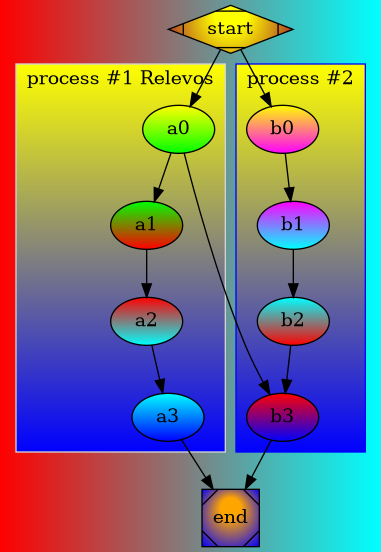
\includegraphics[width=\linewidth]{ciclismo}
\caption{Grafos}
\label{fig:view}
\end{figure*}

\section{Conclusiòn}

Se construye un algoritmo, para relevos pero, es complicado debido a:\\
Es una pregunta ambigua. No se especifico el tipo de etapa a correr. Ruta, ContraReloj, ContraReloj en equipo.\\
Si es ciclismo de Ruta: se plantea las siguientes etapas:
\begin{itemize}
\item[•]Velocidad individual
\item[•]Velocidad por equipos
\item[•]Kilómetro contrareloj
\item[•]Persecución individual
\item[•]Persecución por equipos
\item[•]Carrera por puntos
\item[•]Keirin
\item[•]Scratch
\item[•]Madison
\end{itemize}
Ciclismo de montaña:
\begin{itemize}
\item[•]Campo a través (Cross Country(XC) )
\item[•]Descenso (Downhill)
\item[•]Eslalom (Slalom)
\end{itemize}
Debe existir un algoritmo para cada una de ellas, entonces se construye un algoritmo generico.
\printbibliography

\end{document}
